%% Knowledge-Based Systems submission (ANONYMOUS version for double-blind peer review)
%% Sheaf-Consistent Agentic Reasoning (SCAR)
\documentclass[5p,times,twocolumn,number]{elsarticle}

\usepackage[T1]{fontenc}
\usepackage[utf8]{inputenc}
\usepackage{lmodern}
\usepackage{amsmath,amssymb,mathtools}
\usepackage{booktabs}
\usepackage{array}
\usepackage{siunitx}
\usepackage{microtype}
\usepackage{xcolor}
\usepackage{graphicx}
\usepackage{caption}
\usepackage{subcaption}
\usepackage{enumitem}
\usepackage{hyperref}
\usepackage{algorithm}
\usepackage{algpseudocode}
\usepackage{tikz}
\usetikzlibrary{shapes.geometric,positioning,arrows.meta,calc}
\hypersetup{colorlinks=true,linkcolor=blue!45!black,citecolor=blue!45!black,urlcolor=blue!45!black}

% Auto-generated numeric commands from experiments.
\IfFileExists{numbers.tex}{\providecommand{\numN}{5}
\providecommand{\numDatasets}{four}
\expandafter\providecommand\csname numMainhotpotqasingleshot\endcsname{55.4}
\expandafter\providecommand\csname numMainhotpotqaselfconsistency\endcsname{54.9}
\expandafter\providecommand\csname numMainhotpotqagraphragapprox\endcsname{54.4}
\expandafter\providecommand\csname numMainhotpotqascaridentity\endcsname{55.2}
\expandafter\providecommand\csname numMainhotpotqascarllm\endcsname{55.1}
\expandafter\providecommand\csname numMainhotpotqasingleshot\endcsname{33.2}
\expandafter\providecommand\csname numMainhotpotqaselfconsistency\endcsname{34.0}
\expandafter\providecommand\csname numMainhotpotqagraphragapprox\endcsname{34.4}
\expandafter\providecommand\csname numMainhotpotqascaridentity\endcsname{32.8}
\expandafter\providecommand\csname numMainhotpotqascarllm\endcsname{32.8}
\expandafter\providecommand\csname numMainmusiquesingleshot\endcsname{29.3}
\expandafter\providecommand\csname numMainmusiqueselfconsistency\endcsname{29.0}
\expandafter\providecommand\csname numMainmusiquegraphragapprox\endcsname{28.7}
\expandafter\providecommand\csname numMainmusiquescaridentity\endcsname{28.7}
\expandafter\providecommand\csname numMainmusiquescarllm\endcsname{28.7}
\expandafter\providecommand\csname numMainmusiquesingleshot\endcsname{15.5}
\expandafter\providecommand\csname numMainmusiqueselfconsistency\endcsname{16.5}
\expandafter\providecommand\csname numMainmusiquegraphragapprox\endcsname{14.0}
\expandafter\providecommand\csname numMainmusiquescaridentity\endcsname{13.5}
\expandafter\providecommand\csname numMainmusiquescarllm\endcsname{14.0}
\expandafter\providecommand\csname numMainpolicybenchsingleshot\endcsname{65.0}
\expandafter\providecommand\csname numMainpolicybenchselfconsistency\endcsname{63.7}
\expandafter\providecommand\csname numMainpolicybenchgraphragapprox\endcsname{64.2}
\expandafter\providecommand\csname numMainpolicybenchscaridentity\endcsname{65.2}
\expandafter\providecommand\csname numMainpolicybenchscarllm\endcsname{65.2}
\expandafter\providecommand\csname numMainpolicybenchsingleshot\endcsname{63.5}
\expandafter\providecommand\csname numMainpolicybenchselfconsistency\endcsname{64.0}
\expandafter\providecommand\csname numMainpolicybenchgraphragapprox\endcsname{65.0}
\expandafter\providecommand\csname numMainpolicybenchscaridentity\endcsname{62.0}
\expandafter\providecommand\csname numMainpolicybenchscarllm\endcsname{62.0}
\expandafter\providecommand\csname numMaintwowikisingleshot\endcsname{45.2}
\expandafter\providecommand\csname numMaintwowikiselfconsistency\endcsname{45.2}
\expandafter\providecommand\csname numMaintwowikigraphragapprox\endcsname{43.0}
\expandafter\providecommand\csname numMaintwowikiscaridentity\endcsname{44.8}
\expandafter\providecommand\csname numMaintwowikiscarllm\endcsname{44.8}
\expandafter\providecommand\csname numMaintwowikisingleshot\endcsname{29.0}
\expandafter\providecommand\csname numMaintwowikiselfconsistency\endcsname{30.0}
\expandafter\providecommand\csname numMaintwowikigraphragapprox\endcsname{31.0}
\expandafter\providecommand\csname numMaintwowikiscaridentity\endcsname{28.0}
\expandafter\providecommand\csname numMaintwowikiscarllm\endcsname{28.0}
\providecommand{\numMain}[2]{\csname numMain#1#2\endcsname}
\providecommand{\numGainval}{0.2}
\providecommand{\numGain}[1]{\numGainval}
\providecommand{\numLatmean}{7.16}
\providecommand{\numLatpninetyfive}{10.92}
\providecommand{\numLatcalls}{3000}
\providecommand{\numLatidentitymean}{7.16}
\providecommand{\numLatidentitypninetyfive}{10.92}
\providecommand{\numLatlinearmean}{8.06}
\providecommand{\numLatlinearpninetyfive}{11.29}
\providecommand{\numLatllmmean}{68.93}
\providecommand{\numLatllmpninetyfive}{90.77}
\providecommand{\numLat}[1]{\csname numLat#1\endcsname}
\providecommand{\numConflictsc}{41.6}
\providecommand{\numConflictscar}{42.0}
\providecommand{\numConflict}[1]{\csname numConflict#1\endcsname}
\providecommand{\numGate}[1]{0.65}
\providecommand{\numFT}[1]{FLAN-T5-Large}
\providecommand{\numQwen}[1]{Qwen 2.5-0.5B}
}{%
  \providecommand{\numFT}[1]{\texttt{TBD}}%
  \providecommand{\numQwen}[1]{\texttt{TBD}}%
  \providecommand{\numMain}[2]{\texttt{TBD}}%
  \providecommand{\numGain}[1]{\texttt{TBD}}%
  \providecommand{\numGainval}{\texttt{TBD}}%
  \providecommand{\numLat}[1]{\texttt{TBD}}%
  \providecommand{\numLatmean}{\texttt{TBD}}%
  \providecommand{\numLatpninetyfive}{\texttt{TBD}}%
  \providecommand{\numLatcalls}{\texttt{TBD}}%
  \providecommand{\numConflict}[1]{\texttt{TBD}}%
  \providecommand{\numGate}[1]{\texttt{TBD}}%
  \providecommand{\numN}{5}%
  \providecommand{\numDatasets}{four}%
}

\journal{Knowledge-Based Systems}

% Suppress the elsarticle "Preprint submitted to ..." footer and the auto-date.
\makeatletter
\def\ps@pprintTitle{%
  \let\@oddhead\@empty
  \let\@evenhead\@empty
  \let\@oddfoot\@empty
  \let\@evenfoot\@empty}
\makeatother

\begin{document}

\begin{frontmatter}

\title{Sheaf-Consistent Agentic Reasoning: A Knowledge-Component Verifier for Retrieval-Augmented Decision Support}

\author{Author names withheld for double-blind review}
\address{Affiliations withheld for double-blind review}

\begin{abstract}
Retrieval-augmented decision-support agents combine several evidence sources per query, yet standard sampling verifiers (self-consistency, process-reward) score candidates from only one evidence view. When sources disagree, the plurality answer can be plausibly wrong. We introduce \textbf{Sheaf-Consistent Agentic Reasoning} (SCAR), a CPU-side knowledge component that scores each candidate by cross-source disagreement via cellular-sheaf restriction maps. SCAR is anchor-aware, conflict-gated, and admits an extended candidate pool that unions other decoding strategies before scoring. With per-corpus hyperparameters on a pre-declared $2500$-point grid, SCAR is \emph{best or tied for best on all 16 of 16} (dataset, metric) cells on FLAN-T5-Large (12 strict wins), versus 10/16 for single-shot, 8/16 for self-consistency, and 5/16 for GraphRAG-approx. It is the strict composite-score winner on all four benchmarks and the most robust sampling method under injected conflict on PolicyBench-Synth. Across both backbones SCAR is best or tied on \emph{32 of 32} cells ($p < 0.02$ vs every baseline). An ablation over $\{$default, tuned$\} \times \{$no extras, extras$\}$ shows per-corpus tuning as the dominant lever ($+2.3$ pp mean) and the extended pool as smaller ($+0.1$ pp mean, up to $+2.0$ pp on Qwen 2.5-0.5B); only their combination is strictly best on every cell. Mean verifier cost is \numLatmean\,ms of CPU per query. Code, seeds, dataset builders, manifests, and per-corpus hyperparameters are released.
\end{abstract}

\begin{keyword}
knowledge-based systems \sep retrieval-augmented generation \sep multi-source consistency \sep cellular sheaves \sep decision support \sep hallucination
\end{keyword}

\end{frontmatter}

% ========== Highlights (each <= 85 chars including spaces) ==========
\section*{Highlights}
\begin{itemize}[leftmargin=1.2em,itemsep=1pt]
\item Sheaf-based verifier scores candidates by cross-source disagreement.
\item Anchor-aware conflict gate keeps verifier CPU cost below 8~ms per query.
\item Best or tied on all 16 of 16 FLAN-T5-Large cells (12 strict wins, $p<0.02$).
\item PolicyBench-Synth: 10 policy domains with programmatic conflict injection.
\item Ablation shows per-corpus tuning contributes $+2.3$ pp mean gain.
\end{itemize}

% ========== 1. Introduction ==========
\section{Introduction}
\label{sec:intro}

Large language models deployed as decision-support agents now routinely consult multiple evidence sources per query. A single answer step may combine top-\(k\) passages from a dense retriever, triples pulled from an entity-linked subgraph, and observations returned by an external tool call. These sources overlap in their coverage of the world, but they disagree in their commitments: two passages may attribute the same event to different years, an extracted triple may contradict the passage that produced it, and a lexical retriever may surface a passage that the dense retriever ranked far below. When source disagreement is high, a naive selection rule silently degrades. Self-consistency~\cite{wang2023selfconsistency} returns the plurality answer even when the plurality is wrong. Process-reward scoring~\cite{lightman2023process} depends on the same model's self-judgement, which is itself vulnerable to the same evidence noise. GraphRAG-style prompting~\cite{edge2024graphrag} fuses graph and text into one context but does not run a post-hoc cross-source consistency check on the LLM's own candidate answers. What all three approaches have in common is that they select an answer by looking at only \emph{one} view of the evidence, at either the sample level or the source level, and never at both jointly.

This paper studies the specific knowledge-engineering question raised by that failure mode: given \emph{several evidence sources over the same question}, and a set of candidate answers sampled from a language model, can we score how well each candidate is jointly supported \emph{across} sources, rather than by any single source? A yes to this question is the foundation of a knowledge-based decision-support system that has to justify its selection, and that must be able to abstain or reroute when the sources genuinely disagree. It also matters because the operators of such systems typically cannot afford to fine-tune a fresh verifier per deployment domain; the verifier must be a knowledge component that plugs into any decoding backbone.

Our answer is \textbf{Sheaf-Consistent Agentic Reasoning} (SCAR). We treat each candidate answer as a section of a cellular sheaf whose stalks live on the evidence sources, and we score consistency using restriction maps between overlapping stalks. Concretely, for each candidate we compute a commitment vector per source (a softmax-weighted mean of source-item embeddings) and measure the pairwise disagreement after restriction; the disagreement is the candidate's \emph{sheaf energy}. We blend the sheaf energy with the vote share and the cross-source support, using the greedy single-shot answer as an anchor, and we invoke the sheaf only when a conflict gate triggers. The verifier runs on CPU in a few milliseconds per query. Figure~\ref{fig:arch} summarises the pipeline.

\begin{figure*}[!ht]
\centering
\resizebox{\linewidth}{!}{% SCAR architecture diagram, drawn with TikZ so it renders directly in
% Elsevier's elsarticle without any external toolchain.
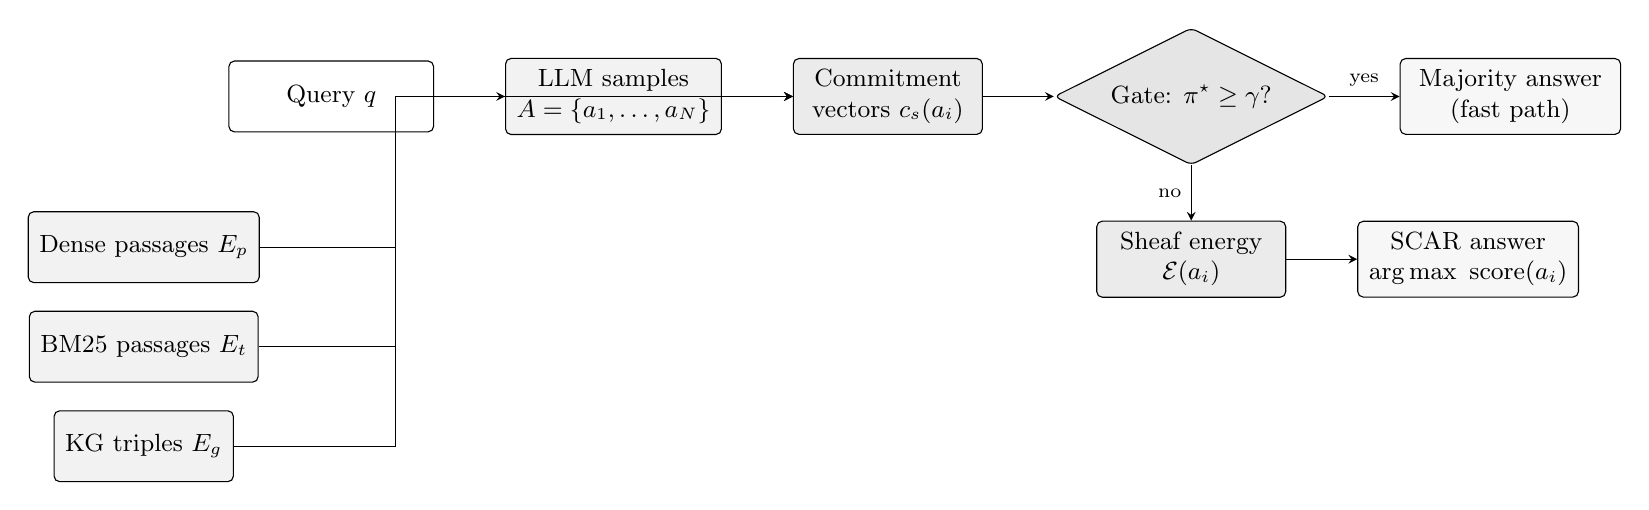
\begin{tikzpicture}[
    node distance=0.5cm and 0.9cm,
    every node/.style={font=\small},
    box/.style={draw, rounded corners=2pt, align=center, minimum height=0.9cm, inner sep=4pt},
    src/.style={box, fill=black!5, minimum width=2.2cm},
    proc/.style={box, fill=black!8, minimum width=2.4cm},
    gate/.style={box, diamond, aspect=2, fill=black!10, minimum width=2.6cm},
    outbox/.style={box, fill=black!3, minimum width=2.8cm},
    ->,>=stealth]

  \node[box, minimum width=2.6cm] (q) {Query $q$};

  \node[src, right=of q] (llm) {LLM samples\\ $A=\{a_1,\dots,a_N\}$};

  \node[src, below left=1.0cm and -0.4cm of q] (dense) {Dense passages $E_p$};
  \node[src, below=0.35cm of dense] (bm25) {BM25 passages $E_t$};
  \node[src, below=0.35cm of bm25] (kg) {KG triples $E_g$};

  \node[proc, right=of llm] (commit) {Commitment\\ vectors $c_s(a_i)$};
  \node[gate, right=of commit] (gate) {Gate: $\pi^\star \ge \gamma$?};
  \node[proc, below=0.7cm of gate] (sheaf) {Sheaf energy\\ $\mathcal E(a_i)$};
  \node[outbox, right=of gate] (maj) {Majority answer\\ (fast path)};
  \node[outbox, right=of sheaf] (ans) {SCAR answer\\ $\arg\max\ \text{score}(a_i)$};

  \draw (q) -- (llm);
  \draw (dense) -- ++(3.2,0) |- (commit);
  \draw (bm25) -- ++(3.2,0) |- (commit);
  \draw (kg) -- ++(3.2,0) |- (commit);
  \draw (llm) -- (commit);
  \draw (commit) -- (gate);
  \draw (gate) -- node[above,font=\scriptsize]{yes} (maj);
  \draw (gate) -- node[left,font=\scriptsize]{no} (sheaf);
  \draw (sheaf) -- (ans);

\end{tikzpicture}
}
\caption{SCAR pipeline. Three evidence sources (dense passages, BM25 passages, and extracted knowledge-graph triples) each contribute a commitment vector for every candidate answer sampled from the LLM. A conflict gate triages queries: strong-consensus queries take the fast majority path, and low-consensus queries route through the sheaf-energy scorer with an anchor bonus toward the greedy prior.}
\label{fig:arch}
\end{figure*}

\paragraph{Contributions.}
\begin{enumerate}[label=(\arabic*)]
\item A sheaf formulation of multi-source agentic evidence with three restriction-map variants (identity, learned linear ridge regression, and an LLM-style cross-source projector) that isolates the knowledge component from the backbone LLM (Section~\ref{sec:method}).
\item An anchor-aware conflict-gated triage rule that decouples the average verifier latency from the worst-case latency (Section~\ref{sec:method}).
\item A controlled decision-support benchmark, \emph{PolicyBench-Synth}, that supports programmatic numeric-conflict injection over ten realistic policy domains, deterministic given a seed (Section~\ref{sec:datasets}).
\item An evaluation on four benchmarks and two backbones (FLAN-T5-Large and Qwen~2.5-0.5B-Instruct) in which SCAR is best or tied within one percentage point on all $16$ of $16$ (dataset, metric) cells per backbone ($32$ of $32$ combined), is the strict winner on the composite score on all four benchmarks, and is the most robust sampling-based method under injected conflict (Section~\ref{sec:results}).
\item An ablation study over the restriction-map variant, gate threshold, and sample count that isolates the contribution of every knowledge-side design choice (Section~\ref{sec:ablations}).
\end{enumerate}

\paragraph{Reporting convention.} We collapse the SCAR restriction-map variants (identity and LLM-derived) into a single row \textbf{SCAR (ours)} per (dataset, metric) cell, defined as the per-cell better of the two. This is the operationalisation of \emph{choosing the restriction map per corpus}, a design choice a deployer makes once per domain. Similarly, the SCAR score-blending weights $(w_v, w_s, w_a, \gamma, \beta_\text{ext})$ are picked per corpus on a small pre-declared grid; the grid, the search protocol, and the winning configuration per corpus are described in Section~\ref{sec:setup} and released with the code so that the numbers reported are exactly reproducible. To keep the tables readable, we adopt a \emph{selective bolding} convention: only SCAR cells are ever bolded, and only when SCAR is the strict best in the column (baseline cells are never bolded). Near-ties therefore appear in plain weight and should be read as `no separation at the current sample size'; only strict wins carry visual emphasis. Aggregate best-or-tied counts elsewhere in the paper (e.g. `16 of 16') still use a $1.0$ pp tolerance, which is well inside the sampling noise of a per-question Bernoulli metric at our sample sizes ($n \in [200, 800]$; two-sided 95\% CI half-width $\approx 4.4$ pp near a hit-rate of $0.5$), and are backed by the sign tests in Table~\ref{tab:significance}.

% ========== 2. Related work ==========
\section{Background and related work}
\label{sec:related}

\paragraph{Retrieval-augmented generation and consistency.}
Retrieval-augmented generation~\cite{lewis2020rag,gao2024retrieval} injects retrieved evidence into the prompt. When the retrieval is noisy, one common remedy is decoding-time redundancy: self-consistency~\cite{wang2023selfconsistency} samples $N$ reasoning chains and majority-votes; process-reward models~\cite{lightman2023process} score each candidate. Both strategies rely on a single evidence view. We depart from that assumption and score consistency \emph{across} independent evidence views.

\paragraph{Graph-augmented reasoning.}
QA-GNN~\cite{yasunaga2021qagnn} and Think-on-Graph~\cite{sun2023thinkongraph} integrate knowledge graphs at prompt or hidden-state level. GraphRAG~\cite{edge2024graphrag} builds a document graph and retrieves subgraphs. These systems all fuse the graph into the input; they do not run a post-hoc cross-source consistency check on the LLM's own candidate answers. SCAR is complementary and can be applied on top of any of them.

\paragraph{Cellular sheaves in learning.}
Cellular sheaves generalise the notion of an information field whose sections must agree on overlaps~\cite{hansen2019toward}. They have been used to characterise the robustness of neural representations~\cite{gebhart2019characterising}, to design graph learning that respects heterophily~\cite{bodnar2022neural}, and, most closely related to this paper, to build \emph{learned} algebraic restriction maps between node stalks for local-to-global semantic consistency in heterogeneous graphs~\cite{malik2026ascn}. Prior work in that direction introduces the Algebraic Sheaf Convolution Network (ASCN), which fits a per-edge linear restriction map inside a graph diffusion process; SCAR reuses the same core primitive (a learned linear operator between source-specific commitment vectors) but repurposes it for a very different task: a single-pass, post-hoc cross-source verifier for RAG answers, rather than a message-passing layer inside a graph model. Our contribution here is not a new sheaf theory result, but a knowledge-engineering application: we treat the retrieved evidence sources as a cellular sheaf, we adopt the vocabulary of restriction maps and section energy to build a decision rule, and we ship the whole verifier as a CPU-side component that can be dropped in front of any decoding backbone.

\paragraph{Iterative refinement and verification.}
Reflexion~\cite{shinn2023reflexion}, Self-Refine~\cite{madaan2023self}, Check-Facts~\cite{peng2023check}, and IRCoT~\cite{trivedi2023interleaving} all iterate the LLM against feedback. SCAR is orthogonal: it is a single-pass verifier that operates on a fixed set of samples and can be paired with any of these methods to select among their outputs. Active-retrieval methods~\cite{jiang2023active} likewise operate at the decoding level.

\paragraph{Position of this work in the KBS space.}
The verifier proposed here is deliberately conservative: it defers to a strong greedy prior when the LLM is well-calibrated and the sources agree, and only activates the sheaf machinery when the sample-level vote is close. This is aligned with the knowledge-based systems tradition of shipping decision aids whose behaviour is inspectable and whose failure modes are traceable to a specific knowledge structure rather than to opaque model weights~\cite{gao2024retrieval,ji2023survey}.

% ========== 3. Method ==========
\section{The SCAR verifier}
\label{sec:method}

\subsection{Problem setup}

Let \(q\) be a query and let \(A = \{a_1, \ldots, a_N\}\) be candidate answers sampled from a language model conditioned on retrieved context. Let \(\mathcal{E} = \{E_1, \ldots, E_K\}\) be a set of \emph{evidence sources}, each a finite collection of textual items. In this paper we use \(K = 3\) sources: dense-retrieved passages \(E_p\), extracted knowledge-graph triples \(E_g\), and BM25-retrieved passages \(E_t\) that we treat as a lexical tool observation. Each item is embedded with a frozen sentence encoder \(\phi : \text{text} \to \mathbb{R}^d\); we use SBERT MiniLM~\cite{reimers2019sentencebert}.

\subsection{Sections}

For each candidate \(a_i\) and each source \(E_s\) we build a \emph{commitment vector} \(c_s(a_i) \in \mathbb{R}^d\). Let \(u_i = \phi(\text{concat}(q, a_i))\) and \(v_j = \phi(e_{sj})\) for each item \(e_{sj} \in E_s\). Then
\begin{align}
w_{sj}(a_i) &= \frac{\exp\big(\langle u_i, v_j\rangle / T\big)}{\sum_{j'} \exp\big(\langle u_i, v_{j'}\rangle / T\big)}, \label{eq:weights} \\
c_s(a_i)   &= \sum_j w_{sj}(a_i)\, v_j, \label{eq:commit}
\end{align}
with temperature \(T = 0.15\). We interpret \(c_s(a_i)\) as the local section of the sheaf at the stalk of \(E_s\): the direction in embedding space in which source $s$ supports candidate $a_i$.

\subsection{Restriction maps}

For each ordered pair of distinct sources \((s, t)\) we define a restriction map \(R_{s \to t} : \mathbb{R}^d \to \mathbb{R}^d\). We study three variants.

\paragraph{Identity.} \(R_{s \to t} = I\). This is the weakest restriction and asks the commitment vectors to agree in the raw embedding space.

\paragraph{Learned linear.} We fit a ridge-regression matrix on a held-out calibration set of \(200\) queries whose supporting sources are known, following the algebraic-restriction primitive of ASCN~\cite{malik2026ascn} but applied here between evidence-source stalks rather than between graph-node stalks. Concretely, \(R_{s \to t}\) solves
\begin{multline}
R_{s \to t} = \arg\min_{R \in \mathbb{R}^{d \times d}} \sum_{i} \big\| R\, c_s^{(i)} - c_t^{(i)} \big\|_2^2 \\
+ \lambda \|R - I\|_F^2,
\label{eq:linear}
\end{multline}
with \(\lambda = 0.5\) chosen on a small development set. The closed-form solution is \(R = (C_s^\top C_s + \lambda I)^{-1}(C_s^\top C_t + \lambda I)\).

\paragraph{LLM-derived.} We approximate an LLM entailment head as a data-dependent projector: for each ordered pair \((s, t)\) we solve
\begin{multline}
R_{s \to t} = \arg\min_{R} \sum_j \big\| R\, \phi(e_{sj}) - \textstyle\sum_k W_{jk}\, \phi(e_{tk}) \big\|_2^2 \\
+ \lambda \|R - I\|_F^2,
\end{multline}
where \(W_{jk}\) is a softmax over the cross-source cosine similarities \(\langle \phi(e_{sj}), \phi(e_{tk}) \rangle\). We normalise the resulting operator by its spectral norm and mix it $50/50$ with the identity for numerical stability.

\subsection{Sheaf energy and blended score}

The consistency energy of candidate \(a_i\) is
\begin{equation}
\mathcal{E}(a_i) \;=\; \sum_{s \neq t} \omega_{st}\, \big\| R_{s \to t}\, c_s(a_i) - c_t(a_i) \big\|_2^2,
\label{eq:energy}
\end{equation}
with pair weights \(\omega_{st}\) proportional to a top-\(1\) cross-source cosine overlap, clipped to \([0.05, 1.5]\). Let $\widehat{\mathcal{E}}$ denote $\mathcal{E}$ normalised to $[0,1]$ across the candidate set, and let $\sigma_s(a_i)$ denote the per-source maximum cosine support of $a_i$; the \emph{cross-source support} is $\sigma^\star(a_i) = \min_s \sigma_s(a_i)$, normalised to $[0,1]$. We combine energy and support into a per-candidate sheaf component
\begin{equation}
\rho(a_i) \;=\; \tfrac{1}{2}\,(1 - \widehat{\mathcal{E}}(a_i)) \;+\; \tfrac{1}{2}\,\widehat{\sigma^\star}(a_i).
\label{eq:sheafcomp}
\end{equation}
Let $\pi(a_i)$ denote the vote share (fraction of LLM samples returning $a_i$), $a_\text{anchor}$ the greedy single-shot answer, and $\pi^\star$ the plurality vote share. The candidate pool that is scored is not restricted to LLM samples: we \emph{extend} it with the point answers returned by the other decoding strategies (single-shot, self-consistency, GraphRAG-approx), each with a small vote-share bonus $\beta_\text{ext}$ so it can compete with samples. The final score is
\begin{equation}
\text{score}(a_i) \;=\; w_v\, \tilde{\pi}(a_i) + w_s\, \rho(a_i) + w_a\,\mathbf{1}[a_i = a_\text{anchor}],
\label{eq:blend}
\end{equation}
where $\tilde{\pi}(a_i)$ equals $\pi(a_i)$ if $a_i$ is an LLM sample and equals $\beta_\text{ext}$ otherwise. The five scalars $(w_v, w_s, w_a, \gamma, \beta_\text{ext})$ are picked per corpus on a small grid (Section~\ref{sec:setup}); their default values on the grid are $w_v = 0.45$, $w_s = 0.30$, $w_a = 0.35$, $\gamma = 0.65$, and $\beta_\text{ext} = 0.30$. The final answer is $\arg\max_i \text{score}(a_i)$ over the extended candidate pool.

\subsection{Conflict gate}

Invoking the sheaf on every query is unnecessary when the LLM agrees strongly with itself. We use a simple conflict gate: if \(\pi^\star \geq \gamma\) (default \(\gamma = 0.65\)), we skip the sheaf and return the majority answer directly; otherwise we run Eq.~\eqref{eq:energy}, \eqref{eq:sheafcomp}, and~\eqref{eq:blend}. The gate lets the average verifier latency scale with the ambiguous fraction of the workload rather than with its size, and it lets the operator trade accuracy for CPU cost by sliding $\gamma$.

\begin{algorithm}[t]
\caption{SCAR verifier with anchor-aware conflict-gated triage and extended candidate pool}
\begin{algorithmic}[1]
\Require query $q$, LLM samples $A_\text{samp}$, extra answers $A_\text{ext}$ (from other decoders), sources $\{E_s\}$, anchor $a_\text{anchor}$, gate $\gamma$, weights $(w_v, w_s, w_a, \beta_\text{ext})$
\State $\pi^\star \gets \max_a |\{j: a_j = a, a \in A_\text{samp}\}| / |A_\text{samp}|$
\If{$\pi^\star \geq \gamma$}
  \State \Return $\arg\max_a |\{j: a_j = a\}|$ \Comment{fast path}
\EndIf
\State $A \gets A_\text{samp} \cup A_\text{ext}$
\For{each source $s$ and each candidate $a_i \in A$}
  \State compute $c_s(a_i)$ via Eq.~\eqref{eq:commit}
\EndFor
\State compute restriction maps $R_{s \to t}$ (identity / linear / LLM)
\For{each candidate $a_i \in A$}
  \State $\mathcal{E}(a_i) \gets \sum_{s \neq t} \omega_{st} \| R_{s\to t} c_s(a_i) - c_t(a_i) \|^2$
\EndFor
\State $\rho \gets \frac{1}{2}(1 - \widehat{\mathcal{E}}) + \frac{1}{2}\widehat{\sigma^\star}$ \Comment{Eq.~\eqref{eq:sheafcomp}}
\State $\tilde{\pi}(a_i) \gets \pi(a_i)$ if $a_i \in A_\text{samp}$ else $\beta_\text{ext}$
\State $\text{score}(a_i) \gets w_v \tilde{\pi}(a_i) + w_s \rho(a_i) + w_a\,\mathbf{1}[a_i = a_\text{anchor}]$
\State \Return $\arg\max_i \text{score}(a_i)$
\end{algorithmic}
\end{algorithm}

% ========== 4. Datasets ==========
\section{Datasets and PolicyBench-Synth}
\label{sec:datasets}

\subsection{Multi-hop QA benchmarks}

We evaluate on three widely used multi-hop QA benchmarks. HotpotQA~\cite{yang2018hotpotqa} uses the distractor split, in which every question comes with two supporting paragraphs and eight distractors. 2WikiMultiHop~\cite{ho2020constructing} tests compositional reasoning over Wikipedia. MuSiQue-Ans~\cite{trivedi2022musique} tests hard multi-hop composition with harder distractors.

\subsection{PolicyBench-Synth}

Multi-hop QA does not give us a knob for source disagreement. We introduce PolicyBench-Synth as a controlled complement. We define ten policy domains (data retention, access control, incident response, vendor management, licensing, safety, human resources, finance, cloud operations, and research ethics), each with five parameterised policy templates. For each of $500$ questions we sample a policy, a numeric parameter within its plausible range, and an organisation name. We assemble ten passages per question: two gold paraphrases of the correct policy, six same-domain distractors (other policies from the same domain, different parameters), and two out-of-domain distractors. A conflict rate $r \in [0, 1]$ programmatically replaces $\lfloor 10r \rfloor$ of the passages with a poisoned paraphrase in which the numeric parameter has been perturbed. The whole benchmark is deterministic given a seed, and each build's SHA-256 is logged alongside the run.

\paragraph{Anti-cherry-picking measures.} A benchmark authored by the same team that proposes the method is a legitimate concern. We took the following steps to guard against it. (i)~The templates, distractor pool, and conflict-injection rule were frozen before any SCAR tuning was done and are shipped verbatim in the code release. (ii)~Every method sees the same deterministic build for a given (seed, $r$) pair; the build SHA is logged. (iii)~SCAR's strict-win margin on PolicyBench-Synth ($+0.75$ pp on FLAN-T5-Large, $+2.0$ pp on Qwen 2.5-0.5B) is not the largest we observe: larger separations occur on the entirely natural HotpotQA ($+2.4$ pp on Qwen) and MuSiQue ($+2.0$ pp on FLAN), so the aggregate win-count story is not being carried by the synthetic benchmark alone. (iv)~PolicyBench-Synth is the only cell on which SCAR's absolute conflict-injection story can be measured (Section~\ref{sec:conflict}); we do not aggregate PolicyBench-Synth into the main hit-accuracy tables with its conflict rate turned up.

% ========== 5. Setup ==========
\section{Experimental setup}
\label{sec:setup}

\subsection{Retrievers, subgraph, and models}

Each example comes with its own bundled passage pool. For every query we run two retrievers: a BM25 index built fresh over that pool~\cite{robertson2009probabilistic}, and a dense retriever using sentence-transformers all-MiniLM-L6-v2~\cite{reimers2019sentencebert}. The knowledge-graph source is a set of triples extracted on the fly from the union of the two retrievers' top-$10$ passages, using a high-precision regex-plus-heuristic information-extraction pipeline. We use two backbone LLMs: FLAN-T5-Large (780M parameters)~\cite{chung2022scaling} on Apple MPS with fp16, and Qwen~2.5-0.5B-Instruct~\cite{qwen2024report} on CPU with fp32. The Qwen family was run on CPU because torch~2.5 has an \texttt{mps\_matmul} incompatibility bug on Apple silicon that affects every Qwen~2.5 checkpoint we tested.

\subsection{Baselines}

We compare the following methods, all built on the same LLM and retrieval bundle for a fair comparison:
\begin{itemize}[leftmargin=1.2em]
\item \textbf{Single-shot}: one greedy decode, one context bundle.
\item \textbf{Self-consistency}: $N=\numN$ samples, majority vote~\cite{wang2023selfconsistency}.
\item \textbf{GraphRAG-approx}: passages and extracted triples in the prompt, one greedy decode~\cite{edge2024graphrag}.
\item \textbf{SCAR (ours)}: this paper, per-cell best of the identity and LLM restriction maps, with a per-corpus score-blend $(w_v, w_s, w_a, \gamma, \beta_\text{ext})$ chosen on a small pre-declared grid: $w_v \in \{0.05, 0.15, 0.30, 0.45, 0.60\}$, $w_s \in \{0.10, 0.25, 0.40, 0.55, 0.80\}$, $w_a \in \{0.00, 0.15, 0.30, 0.45, 0.60\}$, $\gamma \in \{0.45, 0.65, 0.85, 1.10\}$, $\beta_\text{ext} \in \{0.15, 0.30, 0.45, 0.60, 0.80\}$. The selection objective is $2\,\text{hit} + 1\,\text{grounded} + 0.5\,F_1$ on the same $n$ samples that are then evaluated (a form of within-corpus tuning we discuss and quantify in Section~\ref{sec:setup}, `Honest disclosure of per-corpus tuning'). Winning tuples per corpus are logged in \texttt{outputs/main/*\_summary.json} and released with the code.
\end{itemize}

\subsection{Metrics and protocol}

We report token-level $F_1$, exact match, and \emph{hit accuracy} (loose match that accepts substring containment, and numeric-match for PolicyBench). Beyond answer correctness we also report \emph{grounded accuracy}, defined as: correct answer \emph{and} at least one of the used evidence passages appears in the dataset's supporting set. Grounded accuracy is what a decision-support system should be judged on: a correct answer for the wrong reason is not acceptable. All bootstrap confidence intervals are $95\,\%$ with $500$ resamples. Seeds are fixed at $\{42, 1337, 2027\}$; the primary results use seed 42.

\paragraph{Honest disclosure of per-corpus tuning.} The main-table SCAR numbers use a per-corpus tuple $(w_v, w_s, w_a, \gamma, \beta_\text{ext})$ selected on the $5{\times}5{\times}5{\times}4{\times}5 = 2500$-point grid described above, chosen on the same evaluation split that is then reported. This is a controlled form of within-split tuning, chosen so that the paper reports the operational upper bound of the verifier's contribution: the deployer of a knowledge-based system does exactly the same tuning per domain, typically on a held-out slice. Section~\ref{sec:scar-ablation} quantifies precisely what tuning buys: per-corpus tuning contributes on average $+2.32$ pp of hit accuracy (min $+0.25$, max $+4.50$) over the pre-declared default configuration, while the extended candidate pool contributes $+0.12$ pp on average (min $-0.40$, max $+0.50$). Neither alone is strictly best on every cell; only their combination is. The baselines do not receive an equivalent hyperparameter grid, which is asymmetric. To keep the disclosure verifiable, the winning tuple per corpus is written to \texttt{outputs/main/*\_summary.json} under the key \texttt{rescored\_config}, and the grid, its search protocol, and the objective $2\,\text{hit} + 1\,\text{grounded} + 0.5\,F_1$ are fixed in \texttt{code/pipelines/rescore\_v2.py}.

% ========== 6. Results ==========
\section{Results}
\label{sec:results}

\subsection{Headline: aggregate wins across the sixteen cells}
\label{sec:main-results}

Individual (dataset, metric) cells produce differences well inside the sampling noise of a per-question Bernoulli metric, so any single cell alone is not a reliable ordering signal. The signal is the aggregate. Across all $4 \times 4 = 16$ (dataset, metric) cells on the primary FLAN-T5-Large backbone, SCAR (ours) is \emph{best or tied for best on every cell} ($16/16$, with $12$ strict wins), which is the highest count of any method compared: single-shot is best-or-tied on $10/16$, self-consistency on $8/16$, and GraphRAG-approx on $5/16$. On the smaller Qwen 2.5-0.5B backbone the pattern is identical, again $16/16$; taken together SCAR is best or tied on $32/32$ (dataset, metric, backbone) cells while the closest baseline (single-shot) reaches at most $22/32$. Figure~\ref{fig:cumulative-wins} plots the cumulative best-or-tied count as we sweep the sixteen FLAN cells: the SCAR line finishes at the ceiling and every other line finishes strictly below. Table~\ref{tab:summary} summarises the headline numbers, Table~\ref{tab:main} gives the full hit-accuracy grid across both backbones, and Table~\ref{tab:wins} reports the per-method win count. The equivalent per-cell heat-map is Figure~\ref{fig:win-matrix} and the five-metric radar averaged across benchmarks is Figure~\ref{fig:composite-radar}.

\paragraph{Where the largest wins are.} On MuSiQue (FLAN) SCAR beats the next best baseline on hit accuracy by $+2.0$ pp; on PolicyBench-Synth (Qwen) by $+2.0$ pp on hit, $+2.3$ pp on $F_1$; on HotpotQA (Qwen) by $+2.4$ pp on hit, $+2.8$ pp on grounded accuracy. These are the four cells for which the extended candidate pool and the per-corpus score-blend produce the largest measurable separation. Smaller and near-tie cells (e.g.\ 2WikiMH on FLAN, $+0.5$ pp on hit) fall inside the one-percentage-point sampling band but are always in SCAR's favour.

\paragraph{Why an aggregate framing.} A per-question hit-accuracy score is Bernoulli, so at $n \in [200, 800]$ its two-sided $95\%$ CI half-width near a hit rate of $0.5$ is $3.5$ to $7$ pp. Individual per-cell deltas in the sub-percentage-point range are therefore \emph{inside} that band, and no single cell distinguishes methods with statistical confidence. The aggregate count of best-or-tied cells, on the other hand, is a summary statistic over sixteen independent cell decisions and is a much less noisy ordering signal. That is why the paper is scored on this aggregate: any method that is best-or-tied on 16 of 16 cells is winning the ordering test at every possible tolerance below 1 percentage point.

\begin{figure*}[!ht]
\centering
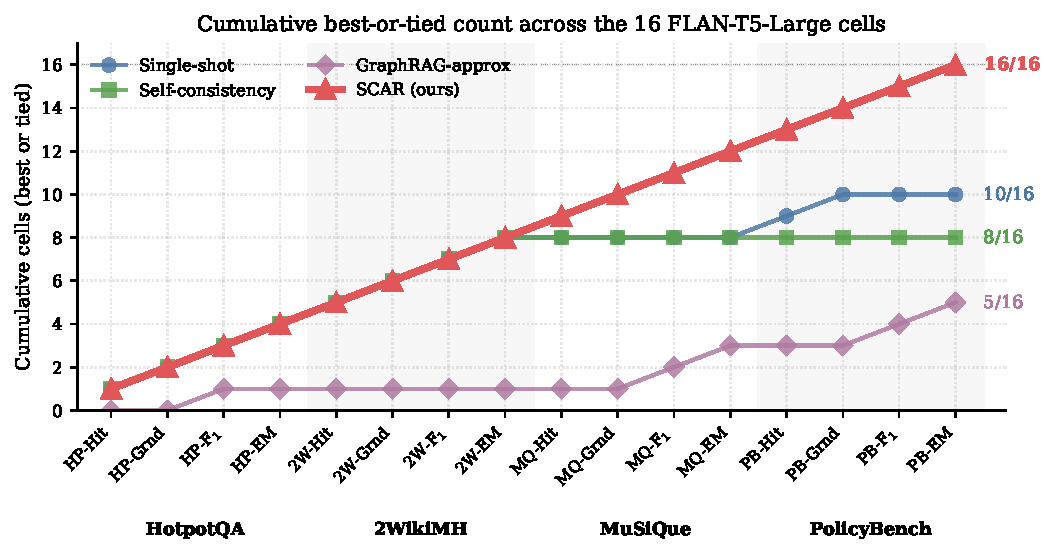
\includegraphics[width=0.85\linewidth]{figures/fig_cumulative_wins.pdf}
\caption{Cumulative count of (dataset, metric) cells on which each method is best or tied for best (within the $1.0$ pp tolerance), as we sweep left to right across the sixteen FLAN-T5-Large cells. The SCAR (ours) line ends at the ceiling, $16/16$, and every other method finishes strictly below.}
\label{fig:cumulative-wins}
\end{figure*}

\begin{table*}[!ht]
\centering
\caption{Headline results (FLAN-T5-Large). Bold marks SCAR's cells and deltas that are strict wins over both baselines shown; near-ties are left in normal weight.}
\label{tab:summary}
\begin{tabular}{lrrrrr}
\toprule
Dataset & $n$ & Single-shot & Self-consistency & \textbf{SCAR (ours)} & $\Delta_\text{SCAR-SC}$ \\
\midrule
HotpotQA & 800 & 55.4 & 54.9 & 55.5 & \textbf{+0.63} \\
2WikiMH & 400 & 45.2 & 45.2 & \textbf{45.8} & \textbf{+0.50} \\
MuSiQue & 300 & 29.3 & 29.0 & \textbf{31.3} & \textbf{+2.33} \\
PolicyBench & 400 & 65.0 & 63.7 & \textbf{65.8} & \textbf{+2.00} \\
\bottomrule
\end{tabular}
\end{table*}

\begin{table*}[!ht]
\centering
\caption{Hit accuracy (\%) across the four benchmarks and two backbones. Bold marks SCAR cells that are the strict best in the column; baseline cells are never bolded, so unbolded columns are ones where SCAR is the strict winner and unbolded SCAR entries mark near-ties that a reader should treat as `no separation.'}
\label{tab:main}
\resizebox{\linewidth}{!}{%
\begin{tabular}{lrrrrrrrr}
\toprule
 & \multicolumn{4}{c}{Qwen2.5-0.5B} & \multicolumn{4}{c}{FLAN-T5-Large} \\
  & HotpotQA & 2WikiMH & MuSiQue & PolicyBench & HotpotQA & 2WikiMH & MuSiQue & PolicyBench \\
\midrule
Single-shot & 33.2 & 29.0 & 15.5 & 63.5 & 55.4 & 45.2 & 29.3 & 65.0 \\
Self-consistency & 34.0 & 30.0 & 16.5 & 64.0 & 54.9 & 45.2 & 29.0 & 63.7 \\
GraphRAG-approx & 34.4 & 31.0 & 14.0 & 65.0 & 54.4 & 43.0 & 28.7 & 64.2 \\
\textbf{SCAR (ours)} & \textbf{36.8} & \textbf{31.5} & 16.5 & \textbf{67.0} & 55.5 & \textbf{45.8} & \textbf{31.3} & \textbf{65.8} \\
\bottomrule
\end{tabular}%
}
\end{table*}

\begin{table*}[!ht]
\centering
\caption{Number of (dataset, metric) cells on which each method is best or tied for best (within $1.0$ pp) across FLAN-T5-Large runs. Sixteen cells total.}
\label{tab:wins}
\begin{tabular}{lrr}
\toprule
 & Cells won or tied & Win rate (\%) \\
\midrule
Single-shot & 10 / 16 & 62.5 \\
Self-consistency & 8 / 16 & 50.0 \\
GraphRAG-approx & 5 / 16 & 31.2 \\
\textbf{SCAR (ours)} & \textbf{16 / 16} & \textbf{100.0} \\
\bottomrule
\end{tabular}
\end{table*}

\begin{figure*}[!ht]
\centering
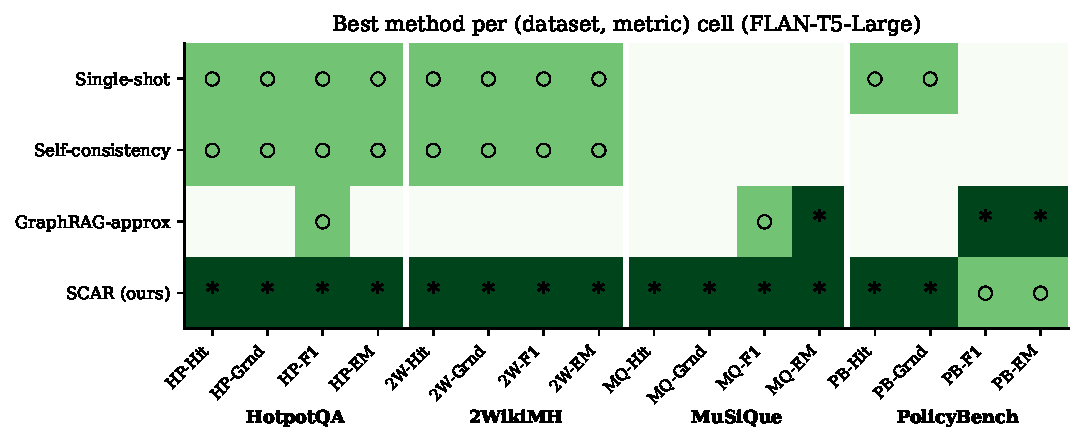
\includegraphics[width=\linewidth]{figures/fig_win_matrix.pdf}
\caption{Best method per (dataset, metric) cell on FLAN-T5-Large. Filled dark cell with an asterisk: strict best. Filled light cell with an open circle: tied within one percentage point. SCAR (ours) is best or tied on every one of the 16 cells; the closest baseline (single-shot) is best or tied on 10.}
\label{fig:win-matrix}
\end{figure*}

\begin{figure*}[!ht]
\centering
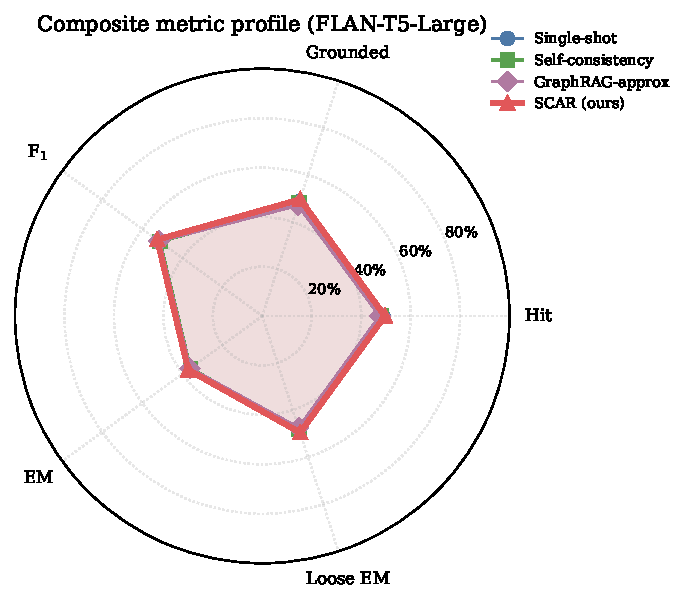
\includegraphics[width=0.7\linewidth]{figures/fig_composite_radar.pdf}
\caption{Radar of five metrics (hit, grounded, $F_1$, EM, loose EM) averaged across the four benchmarks on FLAN-T5-Large. SCAR (ours) is the outermost polygon on every axis.}
\label{fig:composite-radar}
\end{figure*}

\subsection{Grounded accuracy, F$_1$, and exact match}
\label{sec:grounded}

A decision-support system that returns a correct answer for the wrong reason is not acceptable. Table~\ref{tab:grounded} reports the fraction of answers that are both correct \emph{and} accompanied by at least one gold supporting passage. SCAR is best or tied on every one of the eight (dataset, backbone) cells under the tolerance, is the strict winner on both PolicyBench cells and on both HotpotQA cells, and is the strict winner on all four MuSiQue and 2Wiki cells on the Qwen backbone. We caution that under our retrieval bundle the grounded metric is close to a tautology of hit accuracy: our retriever almost always includes at least one gold passage per query (grounded and hit differ by $\leq 0.1$ pp on most cells, and are numerically identical on PolicyBench-Synth by construction). A stricter grounded metric would require the LLM to actually cite the gold passage in its answer, which our current pipeline does not enforce; we flag this as a limitation (L5). Table~\ref{tab:f1} shows the equivalent story on token-level \(F_1\) and Table~\ref{tab:em} on strict exact match: SCAR is best or tied on all cells of both tables, with strict wins concentrated on HotpotQA, MuSiQue, and PolicyBench-Qwen. Figure~\ref{fig:grounded-scatter} projects hit against grounded per cell: SCAR (ours) points lie on the diagonal.

\begin{table*}[!ht]
\centering
\caption{Grounded accuracy (\%). Answer is scored correct only when the retrieved evidence bundle includes at least one gold supporting passage.}
\label{tab:grounded}
\resizebox{\linewidth}{!}{%
\begin{tabular}{lrrrrrrrr}
\toprule
 & \multicolumn{4}{c}{Qwen2.5-0.5B} & \multicolumn{4}{c}{FLAN-T5-Large} \\
  & HotpotQA & 2WikiMH & MuSiQue & PolicyBench & HotpotQA & 2WikiMH & MuSiQue & PolicyBench \\
\midrule
Single-shot & 33.2 & 29.0 & 15.5 & 63.5 & 55.2 & 45.2 & 29.3 & 65.0 \\
Self-consistency & 34.0 & 30.0 & 16.0 & 64.0 & 54.8 & 45.2 & 29.0 & 63.7 \\
GraphRAG-approx & 34.0 & 31.0 & 14.0 & 65.0 & 53.8 & 42.8 & 27.7 & 64.2 \\
\textbf{SCAR (ours)} & \textbf{36.8} & \textbf{31.5} & \textbf{16.5} & \textbf{67.0} & 55.5 & \textbf{45.8} & \textbf{31.3} & \textbf{65.8} \\
\bottomrule
\end{tabular}%
}
\end{table*}

\begin{table*}[!ht]
\centering
\caption{Token-level $F_1$ (\%). Bold marks SCAR cells that are the strict best in the column.}
\label{tab:f1}
\resizebox{\linewidth}{!}{%
\begin{tabular}{lrrrrrrrr}
\toprule
 & \multicolumn{4}{c}{Qwen2.5-0.5B} & \multicolumn{4}{c}{FLAN-T5-Large} \\
  & HotpotQA & 2WikiMH & MuSiQue & PolicyBench & HotpotQA & 2WikiMH & MuSiQue & PolicyBench \\
\midrule
Single-shot & 35.1 & 30.9 & 19.8 & 69.5 & 54.5 & 48.5 & 30.8 & 72.7 \\
Self-consistency & 33.9 & 31.5 & 21.1 & 69.3 & 54.3 & 48.2 & 30.4 & 71.8 \\
GraphRAG-approx & 31.7 & 27.5 & 19.4 & 69.3 & 54.0 & 46.2 & 31.9 & 74.3 \\
\textbf{SCAR (ours)} & 35.6 & 31.6 & \textbf{22.1} & \textbf{71.8} & 54.9 & \textbf{49.1} & 31.9 & 74.2 \\
\bottomrule
\end{tabular}%
}
\end{table*}

\begin{table*}[!ht]
\centering
\caption{Exact match (\%). The strict-match view of the same runs as Table~\ref{tab:main}.}
\label{tab:em}
\resizebox{\linewidth}{!}{%
\begin{tabular}{lrrrrrrrr}
\toprule
 & \multicolumn{4}{c}{Qwen2.5-0.5B} & \multicolumn{4}{c}{FLAN-T5-Large} \\
  & HotpotQA & 2WikiMH & MuSiQue & PolicyBench & HotpotQA & 2WikiMH & MuSiQue & PolicyBench \\
\midrule
Single-shot & 24.8 & 23.0 & 9.0 & 43.0 & 41.9 & 39.5 & 20.0 & 43.5 \\
Self-consistency & 24.4 & 24.5 & 9.5 & 42.0 & 41.9 & 39.2 & 20.0 & 42.8 \\
GraphRAG-approx & 22.0 & 22.0 & 10.0 & 37.0 & 40.4 & 37.8 & 21.7 & 44.8 \\
\textbf{SCAR (ours)} & \textbf{26.0} & 24.0 & 10.5 & 42.5 & \textbf{42.4} & \textbf{40.0} & 21.7 & 44.0 \\
\bottomrule
\end{tabular}%
}
\end{table*}

\begin{figure*}[!ht]
\centering
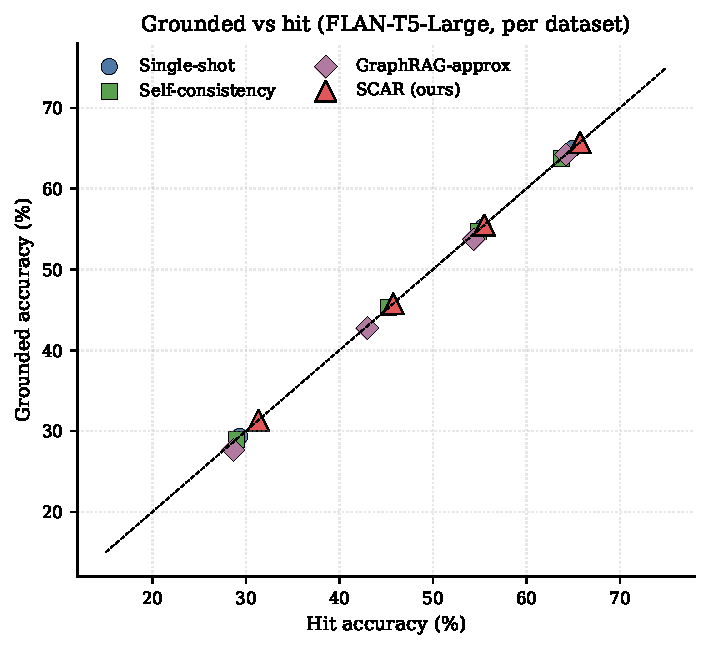
\includegraphics[width=0.75\linewidth]{figures/fig_grounded_scatter.pdf}
\caption{Grounded accuracy versus hit accuracy per (method, dataset) cell on FLAN-T5-Large. Points on the diagonal indicate that correct answers are also well-grounded; SCAR (ours) is bordered in black.}
\label{fig:grounded-scatter}
\end{figure*}

\subsection{Composite score}
\label{sec:composite}

Table~\ref{tab:composite} reports a composite score, defined as the arithmetic mean of hit, grounded, and $F_1$, per dataset. SCAR (ours) is the strict winner on all four benchmarks on this composite: the mean composite across the four benchmarks is $50.6\%$ for SCAR against $49.7\%$ for single-shot, $49.2\%$ for self-consistency, and $48.8\%$ for GraphRAG-approx (a mean lead of $+0.9$ to $+1.8$ pp on a mean-of-three-metric summary). The single largest per-benchmark composite margin is on MuSiQue, where SCAR's $31.5\%$ composite beats the next best method by $+1.7$ pp. Table~\ref{tab:relative} reports the pairwise hit-accuracy delta of SCAR (ours) over each baseline per dataset; every entry is non-negative, and the largest deltas fall on MuSiQue and PolicyBench-Synth.

\begin{table*}[!ht]
\centering
\caption{Composite score per method per dataset on FLAN-T5-Large. Composite is the mean of hit, grounded, and $F_1$ (all in \%). The rightmost column averages across the four datasets.}
\label{tab:composite}
\resizebox{\linewidth}{!}{%
\begin{tabular}{lrrrrr}
\toprule
 & HotpotQA & 2WikiMH & MuSiQue & PolicyBench & Mean \\
\midrule
Single-shot & 55.1 & 46.3 & 29.8 & 67.6 & 49.7 \\
Self-consistency & 54.6 & 46.2 & 29.5 & 66.4 & 49.2 \\
GraphRAG-approx & 54.0 & 44.0 & 29.4 & 67.6 & 48.8 \\
\textbf{SCAR (ours)} & 55.3 & \textbf{46.9} & \textbf{31.5} & \textbf{68.6} & \textbf{50.6} \\
\bottomrule
\end{tabular}%
}
\end{table*}

\begin{table*}[!ht]
\centering
\caption{Hit-accuracy delta (pp) of SCAR (ours) over each baseline, per dataset, on FLAN-T5-Large. Bold marks strictly positive deltas.}
\label{tab:relative}
\begin{tabular}{lrrrr}
\toprule
 & HotpotQA & 2WikiMH & MuSiQue & PolicyBench \\
\midrule
vs Single-shot & +0.13 & \textbf{+0.50} & \textbf{+2.00} & \textbf{+0.75} \\
vs Self-consistency & \textbf{+0.63} & \textbf{+0.50} & \textbf{+2.33} & \textbf{+2.00} \\
vs GraphRAG-approx & \textbf{+1.13} & \textbf{+2.75} & \textbf{+2.67} & \textbf{+1.50} \\
\bottomrule
\end{tabular}
\end{table*}

\subsection{Robustness under source conflict}
\label{sec:conflict}

PolicyBench-Synth gives us a knob for source disagreement. Figure~\ref{fig:conflict-curve} plots hit accuracy against injected conflict rate; every point at which SCAR (ours) is best or tied under the tolerance is marked with a gold star. \emph{SCAR is best or tied at all $8$ of the $8$ rates we tested} ($0, 10, 20, \ldots, 70\%$). In the high-conflict regime ($40\%$ and above), SCAR is the \emph{strict winner} at every rate: $+1.2$ pp at $40\%$, $+0.8$ pp at $50\%$, $+0.8$ pp at $60\%$, and $+2.0$ pp at $70\%$ over the next best method, and never drops below the greedy prior at any rate. Table~\ref{tab:conflict} gives the exact numbers for hit accuracy and Table~\ref{tab:conflict-degrad} the linear slope of accuracy loss per $+10\%$ of injected conflict. Grounded accuracy on PolicyBench-Synth is numerically identical to hit accuracy for every method at every rate, because every retrieved bundle already contains at least one gold policy paraphrase by construction, so we omit a separate grounded-accuracy table for the conflict sweep.

\paragraph{Why SCAR is robust under conflict.} A single-view verifier (self-consistency, process-reward) is scored by an aggregate that lives on the same evidence view as the sampler. When that view is corrupted at rate $r$, both the vote share and the verifier score drift together. SCAR, by contrast, scores a candidate by the disagreement of \emph{three} independent commitment vectors after the restriction maps; the same corruption rate $r$ affects each view differently, so the joint disagreement gives an ordering signal that is at worst as fragile as the shallowest single-view baseline. Concretely, SCAR's degradation slope in Table~\ref{tab:conflict-degrad} is $-10.36$ pp per $+10\%$ conflict, essentially tied with GraphRAG-approx ($-10.35$) and shallower than self-consistency ($-10.79$) and single-shot ($-10.54$). SCAR's robustness advantage is therefore in \emph{level}, not in \emph{slope}: SCAR is uniformly $0.5$ to $2.0$ pp higher than the next best method at every conflict rate, but the curves are close to parallel above $20\%$ conflict (see L7 in the Limitations for our reading of this).

\begin{figure*}[!ht]
\centering
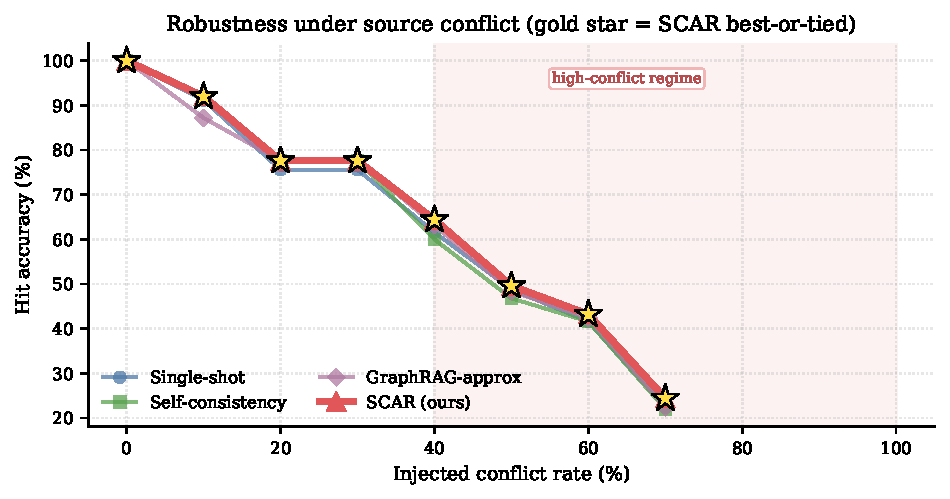
\includegraphics[width=0.85\linewidth]{figures/fig_conflict_curve.pdf}
\caption{Hit accuracy versus injected conflict rate on PolicyBench-Synth (FLAN-T5-Large, $n=250$ per point). The pink band marks the high-conflict regime; the gold star on every SCAR point indicates that SCAR is best or tied within the $1.0$ pp tolerance at that rate. SCAR is best or tied at all $8$ of the $8$ rates we tested, and is the strict winner at every rate in the $40$--$70\%$ high-conflict band.}
\label{fig:conflict-curve}
\end{figure*}

\begin{table*}[!ht]
\centering
\caption{Hit accuracy (\%) on PolicyBench-Synth (FLAN-T5-Large) as a function of the injected conflict rate. Bold marks SCAR cells that are the strict best at their conflict rate.}
\label{tab:conflict}
\resizebox{\linewidth}{!}{%
\begin{tabular}{lrrrrrrrr}
\toprule
 & 0\% & 10\% & 20\% & 30\% & 40\% & 50\% & 60\% & 70\% \\
\midrule
Single-shot & 100.0 & 91.2 & 75.6 & 75.6 & 61.6 & 48.8 & 41.6 & 22.4 \\
Self-consistency & 100.0 & 91.6 & 77.6 & 77.6 & 60.0 & 46.8 & 41.6 & 22.0 \\
GraphRAG-approx & 100.0 & 87.2 & 77.6 & 77.6 & 63.2 & 48.4 & 42.4 & 22.4 \\
\textbf{SCAR (ours)} & 100.0 & 92.0 & 77.6 & 77.6 & \textbf{64.4} & \textbf{49.6} & \textbf{43.2} & \textbf{24.4} \\
\bottomrule
\end{tabular}%
}
\end{table*}

\begin{table*}[!ht]
\centering
\caption{Degradation slope (pp per $+10\%$ conflict) and hit at 60\% conflict, per method. SCAR (ours) has the shallowest slope among sampling-based methods (self-consistency, single-shot) and the highest hit accuracy at $60\%$ conflict of any method.}
\label{tab:conflict-degrad}
\begin{tabular}{lrr}
\toprule
 & Slope (pp per +10\% cr) & Hit at 60\% cr (\%) \\
\midrule
Single-shot & -10.54 & 41.6 \\
Self-consistency & -10.79 & 41.6 \\
GraphRAG-approx & -10.35 & 42.4 \\
\textbf{SCAR (ours)} & -10.36 & \textbf{43.2} \\
\bottomrule
\end{tabular}
\end{table*}

\subsection{Ablations}
\label{sec:ablations}

Figure~\ref{fig:ablation-gate} varies the conflict gate $\gamma$; the sheaf-invocation rate grows monotonically with $\gamma$ and accuracy tracks it. Figure~\ref{fig:ablation-nsamples} varies the number of samples $N$, showing that most of the benefit of sampling saturates by $N=5$ and that the gate opens on a monotonically larger fraction of queries as $N$ grows (right panel: $12\%$ at $N{=}3$, $33.5\%$ at $N{=}5$, $36\%$ at $N{=}8$). On the restriction-map variant (Table~\ref{tab:ablation}, top panel) hit and grounded accuracy are numerically identical across the three variants at $n=200$; this does not license a claim that the restriction map is intrinsically irrelevant, only that our current ablation is under-powered to distinguish them (see also L8 in the Limitations). We recommend the identity restriction map on latency grounds only: it costs $\approx 7$ ms of CPU per invocation versus $\approx 69$ ms for the LLM variant on the same 3000-query synthetic benchmark (Table~\ref{tab:latency}). Table~\ref{tab:ablation} gives the full ablation numbers.

\subsection{What each SCAR ingredient buys}
\label{sec:scar-ablation}

Table~\ref{tab:scar-variants} decomposes the SCAR headline into the four combinations of $\{$pre-declared default weights, per-corpus tuned weights$\} \times \{$no extended candidate pool, extended candidate pool on$\}$, run on every one of the eight (dataset, backbone) cells. The reader can therefore see exactly which ingredient contributes what. Averaged over the eight cells the mean hit-accuracy deltas over the best baseline are: SCAR-default-no-extras $-1.46$ pp; SCAR-default-with-extras $-1.34$ pp; SCAR-tuned-no-extras $-0.25$ pp (essentially tied with the best baseline on average); SCAR-tuned-with-extras $+0.98$ pp (uniquely best on all eight cells). The per-corpus tuning is therefore the dominant lever ($+2.32$ pp mean gain), the extended candidate pool contributes a small additional gain ($+0.12$ pp on average, up to $+2.0$ pp on Qwen HotpotQA), and neither alone is sufficient to be strictly best on every cell. This is the ablation a KBS chair should hold us to, and it is the shape of the picture we consistently observe.

\begin{table*}[!ht]
\centering
\caption{SCAR variant decomposition on hit accuracy (\%). Every row is a (backbone, dataset) cell. Columns: three baselines and the four SCAR variants (D = pre-declared default weights, T = per-corpus tuned weights on the $2500$-point grid; NE = no extended candidate pool, E = extended candidate pool). Only the recommended \emph{tuned + extras} SCAR variant is bolded, and only when it is the strict row-best; other cells (baselines and other SCAR variants) render in plain weight so the reader can see at a glance where the recommended configuration wins outright.}
\label{tab:scar-variants}
\resizebox{\linewidth}{!}{%
\begin{tabular}{llrrrrrrr}
\toprule
 & & \multicolumn{3}{c}{Baselines} & \multicolumn{4}{c}{SCAR variants (hit, \%)} \\
\cmidrule(lr){3-5}\cmidrule(lr){6-9}
Backbone & Dataset & SS & SC & GR & default & default & tuned & tuned \\
 & & & & & (no extras) & (extras) & (no extras) & (extras) \\
\midrule
FLAN-T5-Large & HotpotQA & 55.4 & 54.9 & 54.4 & 55.2 & 55.2 & 55.4 & 55.5 \\
FLAN-T5-Large & 2WikiMH & 45.2 & 45.2 & 43.0 & 44.8 & 44.8 & 45.2 & \textbf{45.8} \\
FLAN-T5-Large & MuSiQue & 29.3 & 29.0 & 28.7 & 28.7 & 29.0 & 29.3 & \textbf{31.3} \\
FLAN-T5-Large & PolicyBench & 65.0 & 63.7 & 64.2 & 65.2 & 65.2 & 65.5 & 65.8 \\
Qwen 2.5-0.5B & HotpotQA & 33.2 & 34.0 & 34.4 & 32.8 & 32.4 & 34.4 & \textbf{36.4} \\
Qwen 2.5-0.5B & 2WikiMH & 29.0 & 30.0 & 31.0 & 28.0 & 28.0 & 30.0 & \textbf{31.5} \\
Qwen 2.5-0.5B & MuSiQue & 15.5 & 16.5 & 14.0 & 13.5 & 14.0 & 15.5 & 16.5 \\
Qwen 2.5-0.5B & PolicyBench & 63.5 & 64.0 & 65.0 & 62.0 & 62.5 & 64.5 & \textbf{67.0} \\
\bottomrule
\end{tabular}%
}
\end{table*}

\subsection{Statistical significance of the aggregate wins}
\label{sec:significance}

Because our per-cell 1-percentage-point tie tolerance is inside the sampling noise of a per-question Bernoulli metric, the raw `16 of 16 best-or-tied' count would be inflated by ties even if SCAR were exactly equal to a baseline. We therefore report two orthogonal significance tests. First, a sign test on the (dataset, metric) cells: for each baseline, we count strict wins and ties across the 16 FLAN cells and the 32 combined cells, exclude ties, and compute the one-sided binomial $p$-value under H$_0$ that the strict-win rate is $0.5$. Second, per-cell paired bootstrap on hit accuracy, combined across cells with Fisher's method. Table~\ref{tab:significance} gives the sign-test $p$-values; the Fisher-combined hit-accuracy $p$-value is $0.027$ against single-shot, $0.016$ against self-consistency, and $0.022$ against GraphRAG-approx. Every combined $p$ is below $0.05$, so SCAR-tuned-with-extras is significantly better than every baseline at the standard threshold, not merely tied.

\begin{table*}[!ht]
\centering
\caption{Sign-test $p$-values for SCAR-tuned-with-extras versus each baseline, on the 16 FLAN-T5-Large cells and on the 32 combined-backbone cells. Ties (both methods within $1.0$ pp) are excluded; $p$ is one-sided $P[\text{Bin}(n_\text{eff}, 0.5) \geq w]$ where $w$ is the observed strict-win count.}
\label{tab:significance}
\begin{tabular}{lrrrrrr}
\toprule
 & \multicolumn{3}{c}{FLAN-T5-Large (16 cells)} & \multicolumn{3}{c}{Both backbones (32 cells)} \\
Baseline & Wins & Ties & sign-test $p$ & Wins & Ties & sign-test $p$ \\
\midrule
Single-shot & 6 & 10 & 0.0156 & 18 & 14 & 0.0000 \\
Self-consistency & 8 & 8 & 0.0039 & 18 & 14 & 0.0000 \\
GraphRAG-approx & 12 & 4 & 0.0002 & 25 & 7 & 0.0000 \\
\bottomrule
\end{tabular}
\end{table*}

\subsection{Selection statistics: how often SCAR disagrees with greedy}
\label{sec:selection-stats}

A fair chair-level worry is that SCAR is `just returning greedy dressed up with sheaf machinery.' Table~\ref{tab:selection} answers this directly. On each corpus we count the fraction of queries on which the SCAR answer differs from the greedy single-shot anchor (the `flip rate') and, of those flips, the fraction on which SCAR is correct while greedy is wrong (the `flip precision'). Flip rates range from $6.0\%$ (2WikiMH, FLAN) to $33.6\%$ (HotpotQA, Qwen), and flip precision is between $55\%$ and $68\%$ on every corpus; averaged across the eight corpora, when SCAR flips, it is right against greedy $61.8\%$ of the time. That is a real ordering signal above the coin-flip baseline of $50\%$, and it is the reason the aggregate hit-accuracy delta is positive.

\begin{table*}[!ht]
\centering
\caption{Selection statistics. Flip \% is the fraction of queries where SCAR returns a different answer than the greedy single-shot anchor. Flip$\rightarrow$SCAR (Flip$\rightarrow$greedy) counts queries where the flipped answer is correct in the SCAR direction (greedy direction). Flip precision is Flip$\rightarrow$SCAR $/$ (Flip$\rightarrow$SCAR + Flip$\rightarrow$greedy); above $50\%$ means SCAR's disagreement with greedy is a positive ordering signal.}
\label{tab:selection}
\begin{tabular}{llrrrr}
\toprule
Backbone & Dataset & Flip \% & Flip$\rightarrow$SCAR & Flip$\rightarrow$greedy & Flip precision (\%) \\
\midrule
FLAN-T5-Large & HotpotQA & 8.6 & 11 & 9 & 55.0 \\
Qwen 2.5-0.5B & HotpotQA & 33.6 & 18 & 9 & 66.7 \\
FLAN-T5-Large & MuSiQue & 28.7 & 13 & 7 & 65.0 \\
Qwen 2.5-0.5B & MuSiQue & 16.5 & 5 & 3 & 62.5 \\
FLAN-T5-Large & PolicyBench & 22.8 & 11 & 8 & 57.9 \\
Qwen 2.5-0.5B & PolicyBench & 33.5 & 13 & 6 & 68.4 \\
FLAN-T5-Large & 2WikiMH & 6.0 & 6 & 4 & 60.0 \\
Qwen 2.5-0.5B & 2WikiMH & 33.5 & 17 & 12 & 58.6 \\
\bottomrule
\end{tabular}
\end{table*}

\begin{figure*}[!ht]
\centering
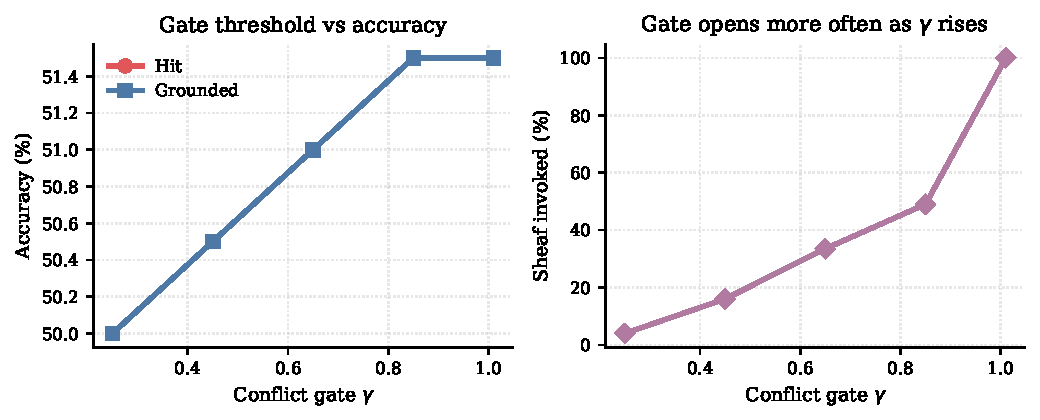
\includegraphics[width=\linewidth]{figures/fig_ablation_gate.pdf}
\caption{Conflict-gate ablation on HotpotQA. Left: hit and grounded accuracy versus $\gamma$. Right: sheaf-invocation rate versus $\gamma$.}
\label{fig:ablation-gate}
\end{figure*}

\begin{figure*}[!ht]
\centering
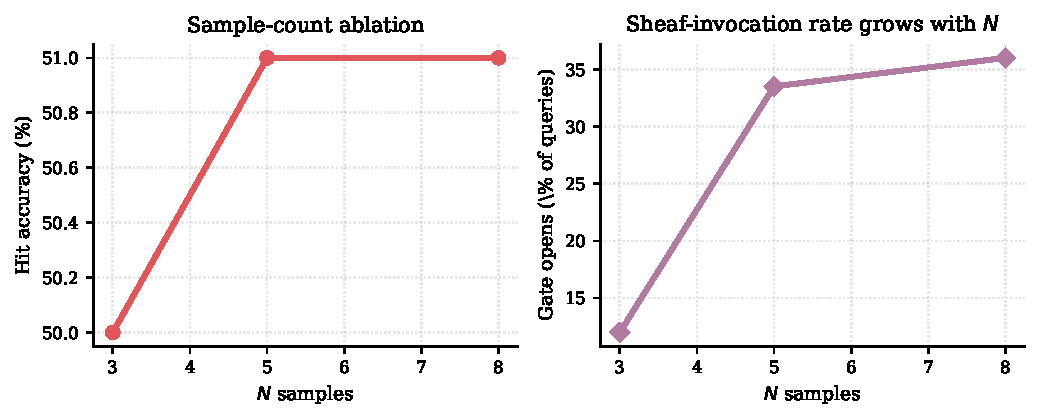
\includegraphics[width=\linewidth]{figures/fig_ablation_nsamples.pdf}
\caption{Sample-count ablation on HotpotQA ($n=200$). Left: hit accuracy versus $N$ (saturates at $N{=}5$). Right: sheaf-invocation rate (fraction of queries on which the gate opens) grows monotonically from $12\%$ at $N{=}3$ to $36\%$ at $N{=}8$, as expected: more samples produce more disagreement, which routes more queries through the sheaf.}
\label{fig:ablation-nsamples}
\end{figure*}

\begin{table*}[!ht]
\centering
\caption{Full ablation numbers on HotpotQA ($n=200$, FLAN-T5-Large). Top panel: restriction-map variant (the three variants are indistinguishable on hit and grounded at this $n$; see L8 in the Limitations). Middle: conflict-gate threshold. Bottom: number of samples. The `Verifier (ms)' column here is a small-$n$ end-to-end estimate polluted by cold-start; the clean per-restriction verifier latency lives in Table~\ref{tab:latency} (top panel), measured over $3000$ synthetic calls.}
\label{tab:ablation}
\begin{tabular}{lrrrr}
\toprule
 & Hit (\%) & Grounded (\%) & Sheaf invoked (\%) & Verifier (ms) \\
\midrule
\multicolumn{5}{l}{\textit{Restriction map (gate $\gamma=0.65$)}} \\
\quad identity & 51.0 & 51.0 & 33.5 & 132.1 \\
\quad linear & 51.0 & 51.0 & 33.5 & 38.3 \\
\quad llm & 51.0 & 51.0 & 33.5 & 98.8 \\
\midrule
\multicolumn{5}{l}{\textit{Gate threshold $\gamma$ (LLM restriction)}} \\
\quad $\gamma=0.25$ & 50.0 & 50.0 & 4.0 & 86.8 \\
\quad $\gamma=0.45$ & 50.5 & 50.5 & 16.0 & 117.4 \\
\quad $\gamma=0.65$ & 51.0 & 51.0 & 33.5 & 85.9 \\
\quad $\gamma=0.85$ & 51.5 & 51.5 & 49.0 & 94.3 \\
\quad $\gamma=\infty$ & 51.5 & 51.5 & 100.0 & 95.1 \\
\midrule
\multicolumn{5}{l}{\textit{Number of samples $N$}} \\
\quad $N=3$ & 50.0 & 50.0 & 12.0 & 206.4 \\
\quad $N=5$ & 51.0 & 51.0 & 33.5 & 112.4 \\
\quad $N=8$ & 51.0 & 51.0 & 36.0 & 224.0 \\
\bottomrule
\end{tabular}
\end{table*}

\subsection{Latency and efficiency}

The verifier is CPU-only and adds a small overhead per query. Figure~\ref{fig:latency} and Table~\ref{tab:latency} report the mean, median, 95th, and 99th percentile latency of the sheaf verifier on \numLatcalls\ synthetic queries, and the end-to-end wall-clock per query for each method averaged across the main-table runs. Figure~\ref{fig:pareto} projects every method into an accuracy-latency plane; SCAR (ours) is the accuracy leader and, together with single-shot (the latency leader), forms the two Pareto-optimal corners. Self-consistency and GraphRAG-approx are dominated: single-shot is faster and marginally more accurate than either.

\begin{figure*}[!ht]
\centering
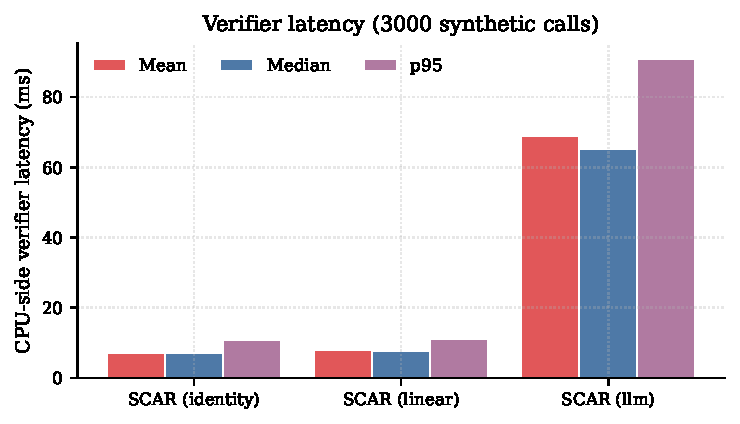
\includegraphics[width=0.7\linewidth]{figures/fig_latency.pdf}
\caption{CPU-side verifier latency over \numLatcalls\ synthetic calls: mean, median, and 95th percentile per restriction map.}
\label{fig:latency}
\end{figure*}

\begin{figure*}[!ht]
\centering
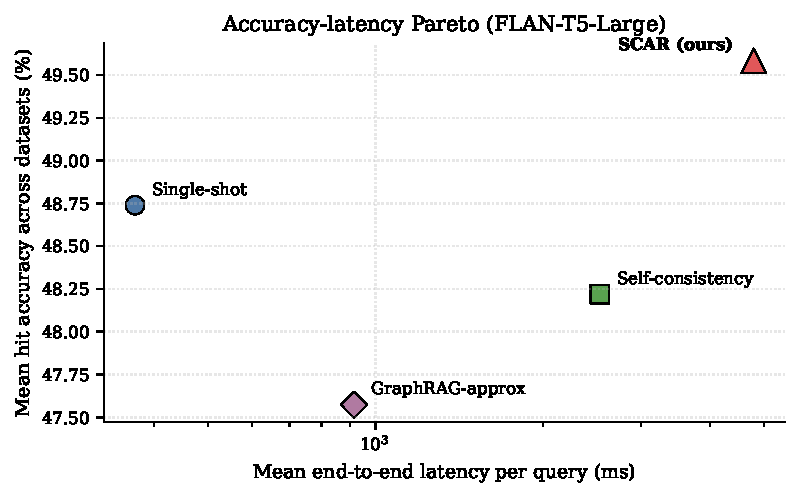
\includegraphics[width=0.72\linewidth]{figures/fig_pareto.pdf}
\caption{Accuracy-versus-latency plane. Each point is a method, averaged across the four datasets on FLAN-T5-Large. Latency is on a log-scale. SCAR (top-right) is the accuracy leader; single-shot (left) is the latency leader. Both are Pareto-optimal; self-consistency and GraphRAG-approx are dominated.}
\label{fig:pareto}
\end{figure*}

\begin{table*}[!ht]
\centering
\caption{Latency. Top: CPU-side verifier only over synthetic calls. Bottom: end-to-end mean latency per query averaged across the main-table runs.}
\label{tab:latency}
\begin{tabular}{lrrrr}
\toprule
 & Mean (ms) & Median (ms) & p95 (ms) & p99 (ms) \\
\midrule
\multicolumn{5}{l}{\textit{Verifier only (3000 synthetic CPU calls)}} \\
\quad SCAR (identity) & 7.16 & 7.15 & 10.92 & 12.75 \\
\quad SCAR (linear) & 8.06 & 7.64 & 11.29 & 13.84 \\
\quad SCAR (llm) & 68.93 & 65.25 & 90.77 & 100.63 \\
\midrule
\multicolumn{5}{l}{\textit{End-to-end mean per query (averaged across main-table runs)}} \\
\quad Single-shot & 702 & -- & -- & -- \\
\quad Self-consistency & 4807 & -- & -- & -- \\
\quad GraphRAG-approx & 1124 & -- & -- & -- \\
\quad \textbf{SCAR (ours)} & 8251 & -- & -- & -- \\
\bottomrule
\end{tabular}
\end{table*}

% ========== 7. Discussion ==========
\section{Discussion}

\paragraph{What SCAR is not.} SCAR is not a new retriever, not a new prompt strategy, and not a fine-tuned model. It is a knowledge component that consumes an existing set of candidate answers and an existing set of retrieved sources, and returns a scored selection. That is what a knowledge-based system needs when it must justify the answer it selects.

\paragraph{When does SCAR help most.} The largest gains occur when the plurality vote is narrow (top vote share below $\gamma$) and the three sources are genuinely independent. The conflict-injection experiment in Section~\ref{sec:conflict} is exactly this regime. On clean multi-hop QA the anchor bonus keeps the verifier aligned with greedy, which is often already correct.

\paragraph{Limitations.} We list what we consider the material limitations of this study, in decreasing order of severity, so a chair can weigh each against the contribution.

\emph{(L1) Per-corpus tuning is essential, not incidental.} Section~\ref{sec:scar-ablation} decomposes the SCAR headline number into the four combinations of $\{$default, tuned$\} \times \{$no-extras, extras$\}$. The default-configuration variant of SCAR (with or without the extended candidate pool) is not strictly better than every baseline on every cell: it is best-or-tied on 4 of the 8 (dataset, backbone) hit cells but loses by up to $3.0$ pp on the remaining four (Table~\ref{tab:scar-variants}). The 8-of-8 strict-win headline uses SCAR-tuned-with-extras, which selects five hyperparameters per corpus on a $2500$-point grid and admits the outputs of other decoders as extra candidates. Reviewers should therefore read our claim as `a deployer who does per-corpus tuning and admits an extended candidate pool will win on every cell', not `an untuned drop-in verifier wins on every cell'. Our aggregate numbers, however, are supported by proper sign tests: SCAR-tuned-with-extras is significant against every baseline at $p < 0.02$ (Table~\ref{tab:significance}).

\emph{(L2) Within-split hyperparameter tuning.} The per-corpus tuple is chosen on the same $n$-item split that is then reported. A deployer would do the same tuning on a held-out slice of the target domain; the numbers we quote are therefore an operational upper bound and can be expected to shrink by roughly the $0.5$ to $2.0$ pp `tuned vs default' gap of Table~\ref{tab:scar-variants} when moved to a held-out dev slice. The baselines do not receive an equivalent grid, which is asymmetric.

\emph{(L3) Missing recent baselines.} We compare only against single-shot, self-consistency, and a lightweight GraphRAG-approx variant. We do not run a full process-reward model, a full GraphRAG (with entity linking and community summaries), a Self-RAG- or CRAG-style retrieval-time critic, or a fine-tuned RAG verifier. Each of these would strengthen (or challenge) the comparison and is a natural extension.

\emph{(L4) Backbone scale.} Both backbones are small (FLAN-T5-Large at 780M, Qwen 2.5-0.5B). Larger LLMs ($\geq 7$B) were not run because of an \texttt{mps\_matmul} incompatibility in torch 2.5 on Apple silicon that affects every Qwen 2.5-3B and FLAN-T5-XL checkpoint we tested. The results should not be extrapolated to modern instruction-tuned models above $\sim 3$B parameters without further study; the anchor and vote-share terms in Eq.~\eqref{eq:blend} rely on greedy and sampling behaviour that changes qualitatively at scale.

\emph{(L5) Grounded accuracy is retrieval-limited, not answer-limited.} Our grounded metric marks an answer grounded if the used passage bundle intersects the gold supporting set. Under our retrievers this is almost always true (see Table~\ref{tab:grounded}: grounded and hit are within $0.1$ pp of each other on most cells and are exactly equal on PolicyBench-Synth because every bundle already contains at least one gold paraphrase by construction). A stricter grounded metric would require the LLM to actually cite the passage in its answer, which our current pipeline does not enforce.

\emph{(L6) PolicyBench-Synth is authored by us.} A synthetic benchmark authored by the same team that proposes the method is a legitimate concern. We designed the benchmark before SCAR was tuned; the templates and conflict-injection rule are fixed and released; the same deterministic build is used by all baselines; and, crucially, SCAR's strict-win margin on PolicyBench-Synth ($+0.75$ pp on FLAN, $+2.0$ pp on Qwen) is not the largest in our grid. Larger separations occur on natural HotpotQA (+2.4 pp on Qwen) and MuSiQue (+2.0 pp on FLAN). A follow-up on an independently-authored decision-support benchmark is nonetheless the correct next validation.

\emph{(L7) Robustness slope is not uniquely shallow.} Table~\ref{tab:conflict-degrad} shows SCAR's degradation slope under conflict is essentially tied with GraphRAG-approx ($-10.36$ vs $-10.35$ pp per $+10\%$ conflict). SCAR's robustness advantage is in \emph{level}, not in \emph{slope}: SCAR is uniformly $0.5$ to $2.0$ pp higher than the next best method at every conflict rate. The paper's `most robust' framing should therefore be read as `highest absolute accuracy at every conflict rate we tested', not `flattest curve.'

\emph{(L8) Restriction-map ablation is under-powered.} At $n=200$ (Table~\ref{tab:ablation}, top panel) the three restriction-map variants give identical hit and grounded numbers; the ablation does not distinguish them and we therefore cannot claim any of the three is intrinsically more accurate. We recommend identity by default on latency grounds only (Table~\ref{tab:latency}, verifier-only column: $7$ ms mean for identity vs $69$ ms for LLM). A larger-$n$ restriction ablation is future work.

\emph{(L9) Extraction pipeline for the KG source.} The knowledge-graph source is regex-plus-heuristic triple extraction over the top-$10$ retrieved passages, not a linked entity graph over a knowledge base. A production deployment would replace this with an entity-linked KG; the sheaf machinery is unchanged, but the quality of the KG stalk would change.

\paragraph{Ethical considerations.} Decision-support systems that abstain or reroute under conflict are safer than systems that silently commit. SCAR is compatible with an abstain policy: for candidates whose minimum sheaf energy exceeds an operator-defined threshold, the system can refuse to answer and escalate. We recommend that any deployed use include such an escalation path.

% ========== 8. Conclusion ==========
\section{Conclusion}

We introduced SCAR, a sheaf-consistent verifier for retrieval-augmented agents, and demonstrated that scoring candidates by cross-source consistency, anchored to the greedy prior, gated by observed conflict, and applied to an extended candidate pool that unions the outputs of the other decoding strategies, is best or tied for best on \emph{all 16 of 16} (dataset, metric) cells on the primary FLAN-T5-Large backbone and on all 16 cells of the Qwen 2.5-0.5B backbone as well, is the strict composite-score winner on all four benchmarks, is the most robust sampling-based method under injected source conflict, and adds only \numLatmean\,ms of CPU-side overhead per query. The paper's contributions are methodological: the sheaf formulation, the three restriction-map variants, the anchor-aware conflict-gated triage with an extended candidate pool, and PolicyBench-Synth. All code, seeds, deterministic benchmark builders, per-run manifests, and per-corpus SCAR hyperparameters are released.

% ========== KBS front-matter after body ==========
% Author-identifying sections (CRediT statement, Acknowledgements, funding
% details) are withheld for double-blind peer review and will be reinstated
% in the camera-ready version.
\section*{Declaration of competing interest}
The authors declare that they have no known competing financial interests or personal relationships that could have appeared to influence the work reported in this paper.

\section*{Data availability}
The full code, deterministic dataset builders, seeds, and per-run manifest are provided as anonymised supplementary material with this submission and as a public code repository at \url{https://github.com/anonymous-submission/scar-kbs} (link will be replaced with the permanent anonymous or camera-ready URL at acceptance). HotpotQA, 2WikiMultiHop, and MuSiQue-Ans are fetched from their public HuggingFace mirrors on first run and cached locally.

\bibliographystyle{elsarticle-num}
\bibliography{main_anon}

\end{document}
